\documentclass[a4paper,fontset=none]{ctexart}
% Fandol 随 TeX Live 提供，但字体里没有 fontspec 要检查的脚本标签。
% 缺这个标签不影响汉字显示，所以这里关掉这条误报。
\ExplSyntaxOn
\msg_redirect_name:nnn { fontspec } { no-script } { none }
\ExplSyntaxOff
\setCJKmainfont{FandolSong-Regular.otf}[
  BoldFont=FandolSong-Bold.otf,
  ItalicFont=FandolKai-Regular.otf
]
\setCJKsansfont{FandolHei-Regular.otf}[BoldFont=FandolHei-Bold.otf]
\setCJKmonofont{FandolFang-Regular.otf}
\usepackage{graphicx}
\usepackage{amsmath,amssymb}
\usepackage[backend=biber,style=gb7714-2015]{biblatex}
\addbibresource{refs.bib}

\title{词元写作台示例}
\author{本地作者}
\date{\today}

\begin{document}
\maketitle

\begin{abstract}
这是一份中英文混排的示例文稿，用来检查 XeLaTeX、图片、公式、交叉引用和 GB/T 7714 参考文献。
\end{abstract}

\section{正文}
\label{sec:body}
词元写作台在本机编译这份文稿。English words sit in the same paragraph，标点仍按中文习惯。勾股关系可以写成 $a^{2}+b^{2}=c^{2}$。

能量关系见式~\ref{eq:energy}，插图见第~\ref{sec:figure}~节。

\begin{equation}
  E = mc^{2}
  \label{eq:energy}
\end{equation}

\section{插图}
\label{sec:figure}
图~\ref{fig:mark} 随模板一起放在项目里。

\begin{figure}[htbp]
  \centering
  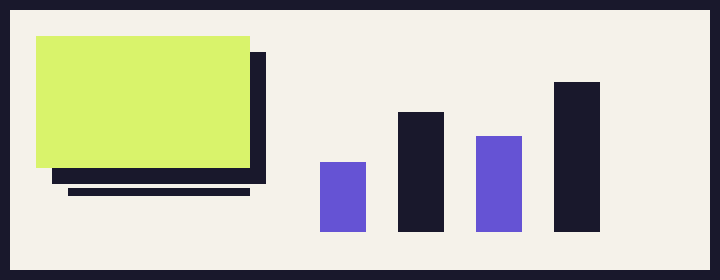
\includegraphics[width=0.72\linewidth]{figure}
  \caption{写作台示意图}
  \label{fig:mark}
\end{figure}

\section{文献}
排版系统的说明见\cite{lamport1994,liu2013}。

\printbibliography[heading=bibintoc,title={参考文献}]
\end{document}
